\documentclass[journal]{IEEEtran}
% IEEE two-column journal format, for IEEE Transactions on Neural Networks and Learning Systems.

\usepackage[T1]{fontenc}
\usepackage{amsmath,amssymb}
\usepackage{booktabs}
\usepackage{graphicx}
\usepackage[numbers,sort&compress]{natbib}
\renewcommand{\bibfont}{\footnotesize}
% let a tall figure with a long caption sit at the top of a text page
\renewcommand{\topfraction}{0.92}
\renewcommand{\textfraction}{0.06}
\renewcommand{\floatpagefraction}{0.85}
\renewcommand{\dbltopfraction}{0.92}
\renewcommand{\dblfloatpagefraction}{0.85}
\usepackage{url}
\usepackage[hidelinks]{hyperref}

\newcommand{\KL}{\mathrm{KL}}

\begin{document}

\title{Equal Weight Error, Unequal Effect: Quantization Sensitivity at the Consuming Operator}

\author{Andrew~H.~Bond,~\IEEEmembership{Senior~Member,~IEEE}%
\thanks{A. H. Bond is with the Department of Computer Engineering, San Jos\'e State University,
San Jos\'e, CA 95192 USA (e-mail: andrew.bond@sjsu.edu; ORCID 0009-0003-2599-6158).}}

\markboth{}{Bond: Quantization Sensitivity at the Consuming Operator}

\maketitle

\begin{abstract}
Weight quantization is often guided by a ranking of a model's components built from
statistics of their weights. We read sensitivity instead at the model's output, operator by
operator, and find that equal weight errors have unequal effects. With one per-output-channel
quantizer at 4 bits, the four attention projections of four language models have similar weight
errors, yet perturbing value and output moves the next-token distribution 2.4 to 3.8 times more
than perturbing query and key. A recently reported ranking puts query and key first. A factorial
on two models traces that ranking to the bit allocation of the shipped llama.cpp presets. The
ordering also depends on the quantizer. A row scale chosen to minimize squared error lowers every
weight error and raises the query-and-key share of the damage, from a ratio of 0.38 to 1.20 on
Llama-3.2-3B and from 0.28 to 0.76 on Qwen2.5-1.5B. GPTQ, which compensates each layer's output
error, keeps the ordering of each row scale on both models. For a key projection, equal error at
the layer's output can mean a ninefold difference at the model's output. Two further operators
show the same dependence. For top-$k$ routers, the ratio of logit-error spread to routing margin
separates a router that keeps its routes at 4 bits from one that loses them. For state-space
models, a 3-bit grid on the logarithm of the decay rate costs 3\% to 35\% in perplexity, while a
grid linear in the rate collapses two Mamba checkpoints, with or without exact grid endpoints.
\end{abstract}

\begin{IEEEkeywords}
Quantization, post-training quantization, large language models, sensitivity analysis, attention,
mixture of experts, state-space models.
\end{IEEEkeywords}

\section{Introduction}\label{sec:intro}

A quantized tensor is usually accepted by one of three checks. Its reconstruction error is
small. The model's accuracy or perplexity stays close to the baseline. Or the component it
belongs to ranks low in a sensitivity order built from weight statistics. The first and third
look at the tensor itself, and the second at an aggregate over the whole model. Methods that use
calibration data go further. GPTQ \citep{frantar2023gptq}, for one, minimizes the error of each
layer's output on calibration inputs. Still, a reconstruction summary or an aggregate score does
not by itself say which directions of an error cause damage at the model's output. That depends
on the operation that reads the tensor.

The cost of leaving that question unasked showed up in an earlier study of key-value cache compression
\citep{anon2026overview}. A per-vector quantizer applied to cached attention keys
reconstructed them better than a 3-bit per-channel quantizer, and its perplexity was 675
times higher. The per-vector quantizer stores each key's norm and quantizes its direction at
4 bits. Normalization alone does not discard the per-channel structure that the attention
score reads, and more directional bits could recover it, so the failure is a misallocation at
a fixed budget. Per-channel key quantization was already known to work
\citep{liu2024kivi,hooper2024kvquant}. The lesson was about acceptance. A reconstruction check
passed a quantizer that the consumer of the tensor could not use.

This paper asks the same question of weight quantization, where precision is often allocated
by a ranking of components. \citet{rababah2026illusion} rank the attention projections by
statistics and divergences of their weights under the quantization schemes of llama.cpp
\citep{gerganov2023llamacpp}, and find the query and key projections the most sensitive.
Section~\ref{sec:proj} gives every projection the same per-output-channel quantizer at the
same bit width and reads sensitivity at the model's output. The relative Frobenius errors of
the four projections are then similar, and the value and output projections move the output
more. Our protocol differs from theirs in bit allocation, quantization scheme and sensitivity
metric at once. Section~\ref{sec:proj:factorial} therefore crosses those factors on two models.
The reported ordering is reproduced by three of five weight statistics under the shipped
presets, and it follows the presets' bit allocation.

Our own ordering is not a property of the projections alone either.
Section~\ref{sec:proj:quant} repeats the 4-bit measurement on two models with a row scale that
minimizes squared error in place of one that covers the row's largest entry. The weight errors
fall and stay equal across the four projections. On Llama-3.2-3B the key projection becomes the
most damaging and the ordering reverses. On Qwen2.5-1.5B the ordering moves most of the way to
parity and does not reverse. Section~\ref{sec:proj:gptq} replaces rounding with GPTQ. Each row
scale then keeps its ordering on both models: value and output dominate under the first scale,
and query and key under the second. What holds under both quantizers, and in the factorial, is the statement in the title:
equal weight errors have unequal effects at the output. Which tensor suffers depends on the
operator that reads it and on the kind of error the quantizer makes.

Below 4 bits the ordering breaks down. Section~\ref{sec:proj:below4} studies one failure, a
3-bit key projection on Llama-3.2-3B under that quantizer. Much of its damage can be removed by
protecting the key rows with the longest rotary wavelengths,
which SpQR had already found sensitive on another model \citep{dettmers2024spqr}. We localize
the damage by wavelength octile on two models and then test the protection against
budget-matched controls on held-out text. The long-wavelength rows are far better to protect
than random rows. They are not the best rows. An eighth chosen by weight error does better on
both models, and we report that against our own earlier reading.

Two further operators show outside attention that the effect of an error depends on where
it falls for the operator that reads it. Section~\ref{sec:route} measures
top-$k$ routers on Mixtral-8x7B and OLMoE-1B-7B, and Section~\ref{sec:decay} measures the decay
of a linear recurrence on two Mamba checkpoints and on RWKV-4. Section~\ref{sec:pullback} states the one definition the four studies share, the output
metric pulled back to the weights, and what would count against the paper's claim.
Section~\ref{sec:agree} gives the decision-level measure, and Section~\ref{sec:trace} a
tracer that assigns each tensor its consuming operator.

We do not offer a better quantizer. We offer measurements of where each operator's fragility
lies, under declared protocols. All experiments use fake quantization on modest samples, and the
claims are relative and directional. Section~\ref{sec:limits} lists what is still missing. The
code repository holds a notebook that rebuilds every reported number from the run records and a
Lean file that checks the paper's identities.

\section{Related work}\label{sec:related}

\paragraph{Beyond aggregate accuracy.} \citet{dutta2024accuracy} showed that compressed models
can match baseline accuracy while many answers flip, proposed the flip count as a distance
between models, and found that KL divergence tracks it. They also count changes from one wrong
answer to another, as AllFlips, and explain flips by small margins between the top answer
options. \citet{rababah2026illusion} introduced Correctness Agreement, the fraction of items
both models answer correctly, together with Cohen's kappa between the two models'
correctness. Our decision-level measure overlaps these closely. Its one addition is a
comparison with a reference perturbation, which we treat as descriptive.

\paragraph{Sensitivity in weight quantization.} Post-training methods such as GPTQ
\citep{frantar2023gptq}, LLM.int8() \citep{dettmers2022llmint8} and SmoothQuant
\citep{xiao2023smoothquant} treat outliers and error compensation. HAWQ
\citep{dong2019hawq,dong2020hawqv2} ranks layers by Hessian curvature to set mixed precision.
SpQR \citep{dettmers2024spqr} found, on LLaMA-65B, that query and key weights tied to
low-frequency rotary components \citep{su2024roformer} are more sensitive than those tied to
high frequencies. Section~\ref{sec:proj:below4} builds on that observation with a localization
by wavelength octile, a quantified intervention and a replication.

\paragraph{Key-value caches.} KIVI \citep{liu2024kivi} and KVQuant \citep{hooper2024kvquant}
quantize keys per channel and values per token.

\paragraph{Mixture-of-experts.} \citet{li2024quantmoebench} found that the components of
mixture-of-experts models differ in their sensitivity to quantization. EAQuant
\citep{fu2025eaquant} observed that small errors in gate scores can change the top-$k$ expert
assignment, and aligns router logits during calibration. We measure how routing flips
distribute over the margin on two real routers.

\paragraph{State-space models.} Quamba \citep{chiang2025quamba} and Quamba2
\citep{chiang2025quamba2} address the quantization of activations and input-dependent
parameters in the selective scan. Mamba \citep{gu2024mamba} already parameterizes its decay
through a logarithm, as earlier diagonal state-space models did \citep{gu2022s4d}. Our
measurement shows what a quantizer that ignores that parameterization does to the model.

\paragraph{Graph-level analysis.} PyTorch's graph-mode quantization builds on torch.fx
\citep{reed2022torchfx}. That capture fails on every library model we tried, so our tracer reads the autograd
graph of one forward pass instead.

\section{Sensitivity as a pulled-back metric}\label{sec:pullback}

The four studies below use four quantities. They are instances of one definition, which we state
once. Let a tensor $W$ be read by an operator $g$, which maps $W$ and an input $x$ to an output
$g(W,x)$ in a space with its own squared distance $d$. The cost of a perturbation $\Delta$ of $W$
is the change it causes at the output, averaged over inputs,
\begin{equation}
S_g(\Delta) = \mathbb{E}_x\, d\bigl(g(W+\Delta,x),\, g(W,x)\bigr).
\label{eq:cost}
\end{equation}
Where $g$ is differentiable in $W$ and $d$ is locally quadratic, the cost of a small perturbation
is a quadratic form,
\begin{equation}
\begin{aligned}
S_g(\Delta) &\approx \mathbb{E}_x \bigl\| D_W g(W,x)[\Delta] \bigr\|^2 = \langle \Delta,\, G\,\Delta\rangle,\\
G &= \mathbb{E}_x\, D_Wg(W,x)^{*} D_Wg(W,x).
\end{aligned}
\label{eq:pullback}
\end{equation}
$G$ is the output metric pulled back to the weights. For a general locally quadratic $d$ the norm
is taken in the Hessian of $d$, which for a KL divergence is the Fisher metric. This is the
Gauss--Newton or Fisher sensitivity that Hessian-based methods already use
\citep{dong2019hawq,frantar2023gptq}, and we claim nothing new in the formula. What we add is the
reading of its degeneracies operator by operator. The Frobenius norm is the special case in
which $G$ is the identity. The directions that $D_Wg$ annihilates are the operator's invariants.
An error along an exact invariant costs nothing at any size, and bits spent resolving it are
wasted. Along a direction that $D_Wg$ merely annihilates, the cost vanishes to second order. The operators of
this paper differ in how $G$ degenerates.

\begin{figure*}[t]
\centering
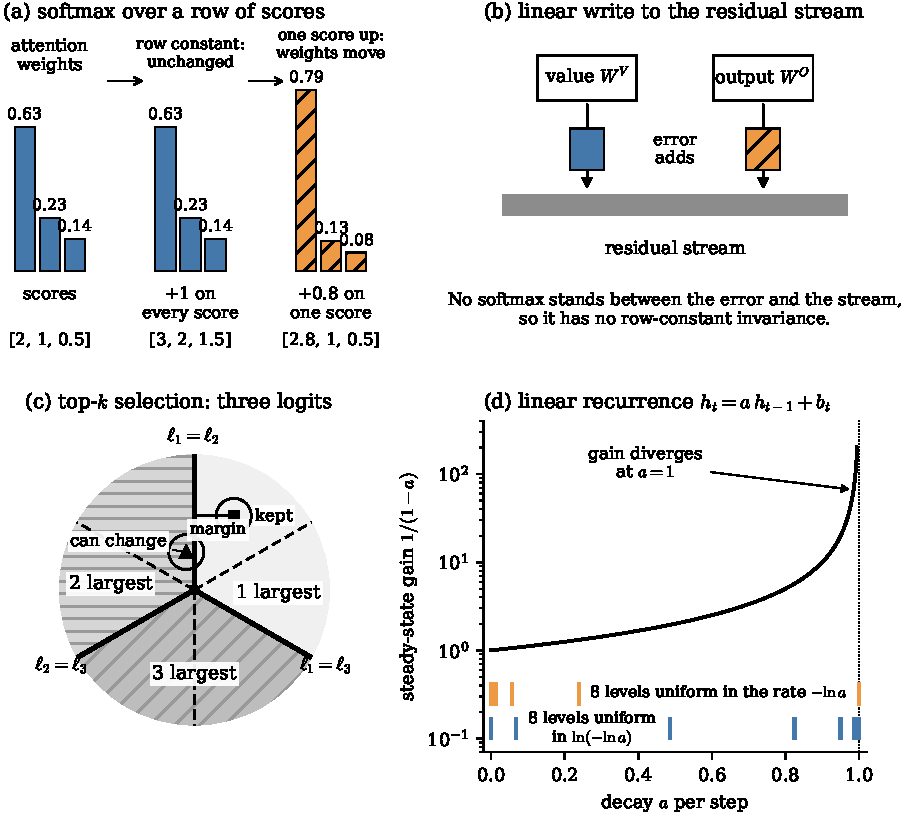
\includegraphics[width=0.62\textwidth]{fig_strata.pdf}
\caption{Each operator treats an error in its own way (a diagram, not a
measurement). (a) A softmax ignores a constant added to a row of scores and responds to a centered
change. (b) Value and output reach the residual stream through linear maps with no softmax in
between, so their error lacks the row-constant invariance of panel (a). Parts of it can still
cancel, in the attention-weighted sum over positions or in a null direction of a later map. (c) A selection changes only when a wall is crossed. Three logits illustrate it; the
routers of Section~\ref{sec:route} have 8 and 64. Solid rays are walls of the top-1 selection,
dashed rays of the top-2 selection. The two circles have the same radius, the size of one perturbation. The bar is the margin
to the nearest top-1 wall, and $R$ compares them: below 1 at the square, above 1 at the triangle.
(d) The gain of a recurrence diverges as the decay $a$ approaches 1. Marks show eight grid levels
for rates between $10^{-3}$ and 10.}
\label{fig:strata}
\end{figure*}

\emph{A linear write.} For $g(W,x) = Wx$ with squared error at the output,
$S_g(\Delta) = \mathbb{E}\|\Delta x\|^2$ exactly, and $G$ is the second-moment matrix of the
inputs acting on each row. Nothing is annihilated unless the inputs are degenerate. This is the
activation-error criterion of Section~\ref{sec:proj:below4} and the layer-wise objective of GPTQ
\citep{frantar2023gptq}, and with whitened inputs it is the Frobenius norm
(Figure~\ref{fig:strata}b).

\emph{A softmax over scores.} The softmax of a row of scores is unchanged when a constant is
added to the row. So $D_Wg$ annihilates every weight perturbation whose score error is constant
along each row, and $G$ sees only the centered part. Section~\ref{sec:proj:factorial} measures
how much of the score error that is (Figure~\ref{fig:strata}a).

\emph{A top-$k$ selection.} Here $g$ is piecewise constant. Its derivative is zero wherever it
exists, so \eqref{eq:pullback} is zero and says nothing, while \eqref{eq:cost} is not zero. The
cost is carried by the tokens that cross a boundary between two selections, and the quantity
that decides it is the distance to that boundary, the margin. The ratio $R$ of
Section~\ref{sec:route} is the perturbation measured in units of that distance. The common-mode
part of a logit error, the part equal on every logit, is again an invariant. In a
mixture-of-experts layer the router's logits also set the mixing weights of the selected
experts through a softmax, so only the selection is piecewise constant, not the whole layer.

\emph{A linear recurrence.} For $h_t = a\,h_{t-1} + b_t$ the steady-state gain is $1/(1-a)$ and
its derivative in $a$ is $1/(1-a)^2$. $G$ does not degenerate here. It diverges as $a$ approaches
1, so equal errors in $a$ cost unequal amounts and a grid should place fine levels near $a=1$.
Under this metric alone the coordinate in which equal steps cost equally is the gain itself.
The logarithm of the decay rate, which equalizes relative error in the rate, also concentrates
its levels there, and a grid uniform in the rate does the opposite (Section~\ref{sec:decay},
Figure~\ref{fig:strata}d).

\paragraph{Selections are stratified.} For the selection operators the right object is not a
metric but a stratification. The hyperplanes $\ell_i = \ell_j$ cut the space of logit vectors
into faces, each given by which logits are tied and the order of the rest. The faces satisfy
Whitney's condition (b), which implies condition (a), so they form a Whitney stratification. The reason
is elementary. Each face is an open piece of a linear subspace, the vectors with its ties, so its
tangent space is that subspace at every point. When a face lies in the closure of another, it has
every tie of the larger face and possibly more, so its subspace is contained in the larger one.
The tangent planes along the larger face are constant and contain the smaller face's tangent
space, which is (a). A secant between a point of each face lies in the larger subspace, which is
closed, so limits of secant directions lie in it, which is (b). The regions on which the selected
set is constant are unions of faces. They are the top strata of a coarser stratification, and we
use the finer one because its strata are flat. Inside a region the selected set
is constant, and it changes only across a wall. A top-$k$ router and the argmax that picks the
next token are the same picture at two places in the model: the margin is $\sqrt2$ times the distance from a
logit vector to the nearest wall that separates selected from unselected, $R$ measures a
perturbation in units of that distance, and the changed predictions of Section~\ref{sec:agree}
are the positions whose output logits cross a wall.

Panel (c) of Figure~\ref{fig:strata} shows the arrangement for three logits. The picture gives a law that can
be checked. Add independent Gaussian noise of scale $\sigma$ to
each logit. The difference of two noises has scale $\sqrt2\,\sigma$, so a token with margin $m$
swaps the pair at its boundary with probability $\Phi(-m/(\sqrt2\,\sigma))$, where $\Phi$ is the
standard normal distribution function. If the margins have density $p$ near zero, then to first
order, counting only the nearest wall,
\begin{equation}
\begin{aligned}
\Pr[\text{the selected set changes}]
&\approx p(0)\int_0^\infty \Phi\!\left(\frac{-m}{\sqrt2\,\sigma}\right)dm\\
&= \frac{p(0)\,\sigma}{\sqrt\pi}.
\end{aligned}
\label{eq:tube}
\end{equation}
Flips grow linearly with the noise scale, at a rate set by how many tokens sit next to a wall.
Section~\ref{sec:route} compares this with the measured noise sweep.

The other two operators are not strata. The softmax is smooth, and its invariance to a row
constant is a symmetry of constant rank, a quotient. The recurrence has a metric that grows
without bound toward $a = 1$, which is a boundary but not a wall that is crossed. We do not claim
a stratification of the space of consumers.

This section is a definition and a way of organizing four measurements. It is not a theorem, and
two limits should be plain. The quadratic form holds for small perturbations of smooth operators, and
the 3-bit failures below are not small. And it treats one operator at a time. In a model the
output of one operator is the input of the next, so the metric that matters at a weight is the
pullback through everything downstream, which is what the KL at the model's output measures and
what we do not decompose. We do not give a rule for composing operators.

\paragraph{What would count against the claim.} Stated loosely, the claim that sensitivity
is set at the consuming operator cannot fail, since \eqref{eq:cost} is defined at the output. It
has content only as a prediction about cheaper proxies. We commit to two. First, a statistic of
the weights alone will misorder tensors that feed different operators, even when their weight
errors are equal. Section~\ref{sec:proj} and the factorial test this. It holds at 8 and 4 bits
under our quantizer and at every level under one K-quant type. At 2 and 3 bits under our
quantizer no ordering is stable, so there it is not tested. Section~\ref{sec:proj:quant} adds a
qualification. Under a second quantizer the weight errors are again equal and the
effects again unequal, so the prediction holds. But on one of two models the order of the two
groups reverses, and there the two projections that feed the softmax differ from each other by a
factor of 8. Under GPTQ it reverses on both (Section~\ref{sec:proj:gptq}). The consumer
does not fix the order. The quantizer's kind of error enters as well. Second, at a
matched budget, a rule derived from the consumer will protect better than a rule that ignores it.
Section~\ref{sec:proj:below4} tests this with the rotary wavelength of the key rows. It holds
against random rows, and it fails against a weight statistic: within the rows of one projection,
which all feed the same operator, the relative weight error of a row selects better than the
wavelength does. It also selects better than the activation-error criterion, which is the
pulled-back metric \eqref{eq:pullback} of the layer's own linear map, on both models. So the evidence supports the claim across operators and does not support it
within one. Inside a single operator a finer weight statistic can be the better proxy for the
cost \eqref{eq:cost}.

\section{Decision-level agreement}\label{sec:agree}

Let $f$ be the base model and $g$ a quantized model, evaluated on $N$ items. The prediction-level
agreement $A = \frac{1}{N}\sum_i \mathbf{1}[f(x_i)=g(x_i)]$ asks whether the two models give the
same answer, right or wrong. Its complement $D = 1-A$ is the fraction of changed predictions, the
AllFlips rate of \citet{dutta2024accuracy}. Accuracy understates it, because regressions and
recoveries cancel in the accuracy change and add in $D$. Correctness Agreement
\citep{rababah2026illusion} equals the base accuracy minus the regressions, so it cannot see
recoveries.

On next-token prediction over the WikiText-2 test split \citep{merity2017pointer}, with every
linear layer in the transformer blocks quantized per output channel at 4 bits, accuracy falls 9.5
points on Qwen2.5-1.5B-Instruct \citep{qwen2025qwen25} while 40.9\% of predictions change, with a
95\% interval of 38.8\% to 42.9\% from resampling whole sequences. On Mistral-7B-v0.1
\citep{jiang2023mistral} a 4.3-point drop comes with 23.2\% of predictions changed, and on
Llama-3.2-3B \citep{grattafiori2024llama3} a 6.7-point drop with 31.9\%. At 8 bits accuracy is
unchanged on all three and 1.2\% to 2.2\% of predictions still change. Section~S-I of the
supplementary material gives the protocol, the full table, and a reference perturbation, an 8-bit
requantization with a small dither, against which the 8-bit changes can be read.

\section{Projection sensitivity at matched bits}\label{sec:proj}

\citet{rababah2026illusion} report that the query and key projections are more sensitive to
quantization than the value and output projections. In its second version (August 2026) the
paper keeps that claim and measures it on Llama-3.2-3B, Vicuna-7B, Mistral-7B and Llama-3.1-8B,
with moments of the weight entries and with divergences between base and quantized weights,
under llama.cpp legacy schemes and K-quant schemes. It reports that the legacy schemes leave
the per-projection statistics almost unchanged and that the distortions in query and key appear
under the 3-bit and 2-bit K-quant schemes. In Section~5 of its first version the paper suggests that future methods allocate higher
precision to query and key and compress value and output more aggressively. Unequal bits across projections are one
candidate explanation for the reported ordering, and the reported metric, a statistic of the
weights rather than of the model's output, is another. Section~\ref{sec:proj:factorial} tests
both.

\paragraph{Protocol.} We quantize $W^Q$, $W^K$, $W^V$ and $W^O$ with the same symmetric absmax
quantizer per output channel, at $b \in \{8,4,3,2\}$ bits. Sensitivity is read two ways. The
weight lens is the relative Frobenius error of each projection. The functional lens perturbs
one projection type in every layer, leaves the rest in full precision, and measures the mean
$\KL(p_{\text{base}}\,\Vert\,p_{\text{quant}})$ of the next-token distribution over
positions, with the top-1 flip rate. The models are Qwen2.5-1.5B-Instruct, Gemma-3-4B-it
\citep{gemma2025gemma3}, Mistral-7B-v0.1 and Llama-3.2-3B, on 24, 16, 32 and 32 WikiText-2
sequences of 256 tokens. The experiment's script records the hypothesis it was written to
confirm, that query and key would move the output more. The result went the other way.

\begin{table*}[t]
\centering
\caption{At matched bits the relative Frobenius errors of the four projections are similar,
while value and output move the output distribution more. Each ratio is the mean over Q and K
divided by the mean over V and O, so a ratio below 1 means query and key move the output less.
Gemma was not run at 2 bits. Brackets are 95\% intervals from a paired bootstrap over whole
sequences.}
\label{tab:proj}
\small
\setlength{\tabcolsep}{4pt}
\begin{tabular}{lcllll}
\toprule
 & rel.\ Frobenius error & \multicolumn{4}{c}{functional $\KL$, ratio QK / VO} \\
\cmidrule(lr){3-6}
model & QK / VO, all $b$ & 8-bit & 4-bit & 3-bit & 2-bit \\
\midrule
Qwen2.5-1.5B & 0.94--1.00 & 0.38 [0.36, 0.40] & 0.26 [0.25, 0.28] & 0.17 [0.17, 0.18] & 0.27 [0.26, 0.27] \\
Gemma-3-4B & 1.03--1.04 & 0.88 [0.82, 0.94] & 0.42 [0.39, 0.45] & 0.41 [0.37, 0.45] & -- \\
Mistral-7B & 1.01--1.13 & 0.28 [0.26, 0.30] & 0.29 [0.27, 0.32] & 0.45 [0.42, 0.47] & 1.05 [1.02, 1.08] \\
Llama-3.2-3B & 1.00--1.05 & 0.39 [0.37, 0.42] & 0.36 [0.34, 0.38] & 2.78 [2.56, 3.01] & 1.13 [1.11, 1.15] \\
\bottomrule
\end{tabular}
\end{table*}

\paragraph{Relative Frobenius errors are similar.} Table~\ref{tab:proj} gives the ratio of the
mean relative Frobenius error over query and key to the mean over value and output. It lies
between 0.94 and 1.13 at every bit width on all four models. The errors themselves are not
small below 8 bits. Under this quantizer, which takes each row's scale from its largest entry
with no clipping, the relative Frobenius error of a projection is about 1\% at 8 bits, 17\% to
21\% at 4 bits, 39\% to 46\% at 3 bits and 90\% to 93\% at 2 bits. Everything below 4 bits in
this paper is a statement about that quantizer.

\paragraph{The functional ordering is different.} At 8 and 4 bits the functional ratio is below
1 on every model, though Gemma's 8-bit ratio of 0.88 rests on KLs near $0.002$ for all four
projections, ten times those of the other models, and may sit at a numerical floor. At 4 bits, perturbing value and output moves the output distribution 3.78
times more than perturbing query and key on Qwen2.5-1.5B, with an interval of 3.54 to 4.03,
2.37 times on Gemma-3-4B (2.20 to 2.59), 3.41 times on Mistral-7B (3.09 to 3.77) and 2.75 times
on Llama-3.2-3B (2.60 to 2.92). No interval at 8 or 4 bits reaches 1. The top-1 flip rates at 4 bits agree. On every
model both value and output flip more tokens than both query and key, for instance 0.075 and
0.048 against 0.034 and 0.036 on Mistral-7B. Under this protocol, compressing value and output
harder than query and key would raise the change in the model's output, not lower it. At 2 bits,
where 68\% to 99.5\% of top-1 tokens flip under a single projection type, the ratio is near 1 on
Mistral and Llama and stays at 0.27 on Qwen.

\subsection{Where the two orderings part}\label{sec:proj:factorial}

Table~\ref{tab:proj} does not show why the reported ordering differs. Three things differ
between the two protocols: the bit allocation, the quantization scheme and the sensitivity
metric. We crossed them on Llama-3.2-3B and Mistral-7B at two llama.cpp levels, \texttt{Q2\_K}
and \texttt{Q3\_K\_M}. Each level has four arms. The first is the preset as shipped, with its
mixture of tensor types. The second applies one K-quant type to every tensor, which
\texttt{llama-quantize} offers as \texttt{--pure}. The third and fourth use our per-output-channel
absmax quantizer, with each projection at the bit width of its tensor type in the shipped preset,
or with every projection at the level's bit width. In each arm we perturb one projection type in
every layer and read both the weight statistics of the original study's kind and the functional
KL of Section~\ref{sec:proj}. The K-quant weights are dequantized from GGUF files, and the
conversion's row permutation is inverted and checked against a 16-bit GGUF that reproduces the
original weights exactly.

The shipped presets do not give the projections equal bits. In the llama.cpp build we used,
\texttt{Q2\_K} puts query and key at the 2-bit type and output at the 3-bit type on both models.
It puts value at the 4-bit type on Mistral-7B and at the 3-bit type on Llama-3.2-3B, because
that choice depends on the model's ratio of attention heads to key-value heads. \texttt{Q3\_K\_M}
puts query and key at the 3-bit type, output at the 4-bit type, and value at the 4-bit type in
all but two layers, where it uses the 5-bit type. So a split of 2 bits for query and key, 4 for value and 3 for output holds for Mistral-7B
and not for Llama-3.2-3B. These allocations are from our own reading of the tensor types in the
files, and \citet{rababah2026illusion} do not list them.

\begin{table*}[t]
\centering
\caption{The weight-statistic ordering follows the bit allocation. Each entry is the
mean over query and key divided by the mean over value and output, so a value above 1 says query
and key are the more distorted or the more damaging. Brackets are 95\% intervals from a paired
bootstrap over 32 sequences. Mistral-7B has no intervals.}
\label{tab:factorial}
\small
\begin{tabular}{lllrrl}
\toprule
 & & & \multicolumn{2}{c}{weight statistics, QK / VO} & functional $\KL$ \\
\cmidrule(lr){4-5}
model & level & arm & rel.\ Frobenius & $|\Delta$kurtosis$|$ & QK / VO \\
\midrule
Llama-3.2-3B & \texttt{Q2\_K} & K-quant, shipped mix & 1.97 & 4.24 & 0.91 [0.84, 1.02] \\
 & & K-quant, equal type & 1.00 & 1.23 & 0.17 [0.15, 0.19] \\
 & & per-channel, shipped bits & 2.27 & 333 & 31.6 [29.9, 33.5] \\
 & & per-channel, equal bits & 1.00 & 1.25 & 1.13 [1.11, 1.15] \\
 & \texttt{Q3\_K\_M} & K-quant, shipped mix & 2.17 & 1.94 & 1.12 [1.07, 1.17] \\
 & & K-quant, equal type & 1.01 & 1.20 & 0.23 [0.22, 0.24] \\
 & & per-channel, shipped bits & 2.42 & 3.62 & 15.3 [14.0, 16.7] \\
 & & per-channel, equal bits & 1.04 & 1.52 & 2.77 [2.55, 3.01] \\
\midrule
Mistral-7B & \texttt{Q2\_K} & K-quant, shipped mix & 2.72 & 6.25 & 1.18 \\
 & & K-quant, equal type & 1.02 & 1.92 & 0.057 \\
 & & per-channel, shipped bits & 3.13 & 205 & 67.3 \\
 & & per-channel, equal bits & 1.01 & 1.47 & 1.05 \\
 & \texttt{Q3\_K\_M} & K-quant, shipped mix & 2.16 & 2.94 & 0.61 \\
 & & K-quant, equal type & 1.01 & 1.02 & 0.17 \\
 & & per-channel, shipped bits & 2.54 & 4.08 & 2.47 \\
  & & per-channel, equal bits & 1.09 & 1.57 & 0.445 \\
\bottomrule
\end{tabular}
\end{table*}

Table~\ref{tab:factorial} gives the outcome, and three things follow from it.

First, the bit allocation moves the weight statistics. Under the shipped mix the relative
Frobenius error of query and key is 2.0 to 2.7 times that of value and output, and the change in
kurtosis is 1.9 to 6.3 times larger. With one type for every tensor the Frobenius ratio is 1.00
to 1.02 and the kurtosis ratio is 1.0 to 1.9. The same holds under our quantizer: 2.3 to 3.1 with
the shipped bits and 1.00 to 1.09 with equal bits. A ranking by these statistics under the
shipped presets therefore ranks the projections by how few bits they were given. The records hold
three more statistics of the original study's kind. One minus the cosine between base and
quantized weights behaves like the Frobenius error, 3.8 to 6.4 under the shipped mix. The change
in skewness does not: under the shipped mix it is 0.54 and 0.77 at \texttt{Q2\_K}, the other way
round, and 8.0 and 8.7 at \texttt{Q3\_K\_M}. A divergence between weight histograms ranges from
0.007 to 1{,}100 across the four shipped-mix arms and we treat it as unusable. So the reported
ordering is reproduced by the Frobenius, cosine and kurtosis statistics and not by all five.

Second, at equal bits under K-quant the metric decides the ordering. The Frobenius errors tie,
the kurtosis ratio stays between 1.0 and 1.9, and the functional ratio is 0.17 and 0.23 on Llama, with intervals of 0.15 to 0.19 and
0.22 to 0.24, and 0.057 and 0.17 on Mistral. Perturbing
value and output moves the output 4 to 17 times more than perturbing query and key. This agrees
with Table~\ref{tab:proj} at 8 and 4 bits, under a different quantization scheme.

Third, the shipped allocation roughly evens out the functional damage. With the presets' extra
bits for value and output, the functional ratio is between 0.61 and 1.18. On Llama its interval
is 0.84 to 1.02 at \texttt{Q2\_K}, which includes parity, and 1.07 to 1.17 at \texttt{Q3\_K\_M}.
On this evidence the
presets' choice to spend more bits on value and output is the right way round.

The scheme matters as well, at low bit widths. Per-output-channel absmax at 2 bits gives a KL
between 2.4 and 5.5 for every projection on both models, where the 2-bit K-quant type gives 0.006
to 0.23, so the per-channel arms at \texttt{Q2\_K} mostly measure collapse. At 3 bits with equal
bits the per-channel ratio is 2.77 on Llama and 0.445 on Mistral, as in
Table~\ref{tab:proj}, the instability of Section~\ref{sec:proj:below4}. That instability
belongs to the per-channel quantizer. Under one K-quant type the ordering is the same at the
2-bit and 3-bit types on both models. The factorial has two models and two
levels, with intervals on one of the models, and we did not run the multiple-choice tasks of the original study. What
it supports is narrow. Under the shipped presets, the weight-statistic ordering is explained by
bit allocation, and it does not carry over to equal bits or to an output-level metric.

\paragraph{Why value and output, a partial test.} A perturbation $\Delta W_K$ of the key weights
changes the score of query position $t$ for source position $s$ by an amount proportional to
$q_t^\top \Delta W_K h_s$, before the rotary embedding. Because $h_s$ varies with the source
token, this error varies across the row of scores, and the softmax cancels only a constant
added to the whole row. Value and output write into the residual stream almost linearly, and
their error reaches the output without passing through a softmax. One hypothesis for the
ordering is that the score errors are partly constant along each row, or small next to the gaps
between scores, so that the softmax suppresses a share of them.

We measured both parts on the four models, perturbing one layer at a time on its own unperturbed
inputs, over 8 sequences. For each query row we split the score error into its row mean and the
centered remainder. At 4 bits the row-constant part carries about half of the squared score
error under a query perturbation, with a median over layers of 0.47 to 0.52 on the four models,
and a quarter to a third under a key perturbation, 0.22 to 0.33. The centered part is small next
to the scores' own spread. Its root mean square is 6\% to 11\% of the within-row deviation of the
scores at 4 bits and 15\% to 24\% at 3 bits, and the attention weights move by a total variation
of 0.02 to 0.06 at 4 bits and 0.06 to 0.13 at 3 bits. So the softmax does cancel a real share of
the query error and a smaller share of the key error, and what remains is small at 4 bits. This
supports the hypothesis without establishing it. On Llama-3.2-3B a rerun
gives intervals from a bootstrap over sequences, and they are narrow. Pooled over layers at 4
bits, the row-constant share is 0.46, with an interval of 0.45 to 0.47, under a query
perturbation and 0.36, with 0.34 to 0.38, under a key perturbation. With 32 sequences in place
of 8 the two shares are 0.46 and 0.35. The other three models have no intervals. The measurement
is local to one layer, and we have not related the centered error to the KL at the model's output across
projections, which is the comparison that would test the account. Gemma-3-4B ran in a different
floating-point format from the other three models, on its text model only.

\subsection{Below 4 bits the per-channel quantizer gives no stable ordering}\label{sec:proj:below4}

At 3 bits two models depart from any ordering. On Llama-3.2-3B the key projection alone gives a
KL of 0.741, against 0.089, 0.125 and 0.174 for query, value and output, while its relative
weight error stays ordinary. Its output movement per unit of relative weight error is 1.71, where
the other projections sit between 0.22 and 0.43. On Qwen2.5-1.5B the output projection rises to
0.624 against 0.183 for value. The fragile projection below 4 bits depends on the model, and the
projection-level weight statistics do not single it out.

For the Llama case an analysis note records a hypothesis. The note was committed together
with the probe's result, so we cannot show that it came first, and we do not claim a
prediction. Damage
from 3-bit quantization of rows of $W^K$ should rise with the rotary wavelength of the row, and
the profile should be comparatively flat on Mistral-7B, which shows no anomaly. SpQR's
observation that low-frequency rotary weights are the sensitive ones points the same way
\citep{dettmers2024spqr}. The probe groups the rows of every key projection into eight octiles
of rotary wavelength, taken from the model's own frequency buffer, and either quantizes only one
octile or quantizes all rows except one octile.

\begin{table*}[t]
\centering
\caption{Much of the 3-bit key damage on Llama-3.2-3B is removed by sparing the
long-wavelength rotary rows. The coupling of damage to wavelength appears on both models, and its
size differs by a factor of 25. Shares are of the summed single-octile KL, and the spared share
is of the joint KL. Brackets are 95\% intervals from a paired bootstrap over 32 sequences. The
control has none.}
\label{tab:wave}
\small
\begin{tabular}{lll}
\toprule
 & Llama-3.2-3B & Mistral-7B (control) \\
\midrule
KL with all key rows at 3 bits & 0.741 [0.670, 0.818] & 0.030 \\
sum of the eight single-octile KLs & 0.173 & 0.031 \\
Spearman correlation of single-octile KL with wavelength & 0.905 [0.786, 0.929] & 0.571 \\
two longest octiles, share of the summed single-octile KL & 72\% [71\%, 74\%] & 79\% \\
KL removed by sparing the longest octile (12.5\% of rows) & 87\% & 49\% \\
wavelengths of the longest octile (tokens) & $2.0$--$8.2\times10^{7}$ & $2.0$--$5.4\times10^{4}$ \\
Spearman correlation of row weight error with wavelength & 0.12 & 0.22 \\
\bottomrule
\end{tabular}
\end{table*}

Table~\ref{tab:wave} gives the outcome. The hypothesis was half right. Damage rises with
wavelength on Llama, with a rank correlation of 0.905 across octiles and an interval of 0.79 to
0.93 over sequences. The single-octile KL of the longest octile is 26 to 35 times that of the
shortest. And sparing the
longest-wavelength eighth of the rows removes 87\% of the joint KL. The control is not flat.
Mistral's much smaller damage also concentrates in its longest-wavelength rows. The coupling is
common to both models, and what differs is its amplitude, a KL of 0.741 against 0.030. Llama-3.2
stretches its rotary frequencies for long context, and its longest wavelengths reach
$8.2\times10^{7}$ tokens against $5.4\times10^{4}$ for Mistral. The rows that carry those
wavelengths are nearly constant over any practical window. Per-row weight error correlates with
wavelength at 0.12 on Llama and at 0.22 on the control, which suffers 25 times less. The damage is
superadditive. The single-octile KLs on Llama sum to 0.173, against 0.741 when all rows are
quantized together, so the spared-octile numbers are the ones that matter for deployment.

\paragraph{A targeted protection.} Keeping the longest-wavelength eighth of $W^K$ rows in full
precision was then validated through a separate implementation on different hardware. The K-only
3-bit KL on Llama-3.2-3B fell from 0.7352 to 0.0994, a recovery of 86.5\% against the 87\% the
probe predicted. These are single runs without intervals. Keeping those rows at 8 bits instead gives the same 0.0994. With one eighth of
the rows at 8 bits and the rest at 3, the key weights average 3.625 bits before scale metadata.
At whole-model 4 bits the protection buys only 2.5\%, from 0.4787 to 0.4668, which fits the
4-bit result above, where value and output dominate.

\paragraph{Are these the right rows?} That result shows that protecting these rows is enough. To
ask whether they are the right rows at that budget, we held the budget at 3.625 bits and changed
only which eighth of the rows of every key projection stays at 8 bits. The conditions are the
longest-wavelength octile, the shortest-wavelength octile, a uniform random eighth of the rows
over five seeds, a random set of rotary frequencies with the structure of an octile over five
seeds, the eighth of rows with the largest relative 3-bit weight error, and the eighth with the
largest output error on calibration activations from 16 training sequences. Evaluation is on 64
sequences of the WikiText-2 validation split, which neither the probe nor the calibration saw.

\begin{table*}[t]
\centering
\caption{At a matched budget of 3.625 bits per key weight, the long-wavelength rows are far better
to protect than random rows, and rows chosen by weight error are better still. Held-out
validation text, 64 sequences. Brackets are 95\% intervals from resampling whole sequences. For
the random conditions the range is over seeds.}
\label{tab:protect}
\small
\begin{tabular}{lrrrr}
\toprule
 & \multicolumn{2}{c}{Llama-3.2-3B} & \multicolumn{2}{c}{Mistral-7B} \\
\cmidrule(lr){2-3}\cmidrule(lr){4-5}
eighth of key rows kept at 8 bits & $\KL$ & removed & $\KL$ & removed \\
\midrule
none (all rows at 3 bits) & 0.781 [0.715, 0.837] & & 0.0279 [0.0263, 0.0297] & \\
shortest wavelength & 0.749 [0.688, 0.812] & 4\% & 0.0262 [0.0248, 0.0277] & 6\% \\
random rows, 5 seeds & 0.491 to 0.732 & 6\% to 37\% & 0.0237 to 0.0248 & 11\% to 15\% \\
random frequencies, 5 seeds & 0.350 to 0.627 & 20\% to 55\% & 0.0238 to 0.0251 & 10\% to 15\% \\
longest wavelength & 0.089 [0.083, 0.095] & 89\% & 0.0137 [0.0128, 0.0147] & 51\% \\
largest activation error & 0.031 [0.030, 0.033] & 96\% & 0.0095 [0.0090, 0.0101] & 66\% \\
largest weight error & 0.028 [0.027, 0.029] & 96\% & 0.0073 [0.0069, 0.0078] & 74\% \\
\bottomrule
\end{tabular}
\end{table*}

Table~\ref{tab:protect} gives the result. Wavelength is a real criterion. On Llama-3.2-3B the
longest-wavelength eighth removes 89\% of the KL, where a random eighth of rows removes 6\% to
37\% and the shortest-wavelength eighth removes 4\%. The paired interval for the difference in
KL between each random seed and the longest octile lies above 0.22 in every case. The earlier
numbers hold up on held-out text: on the probe's own set this run gives 0.741 and 0.099, against
0.781 and 0.089 on the validation split.

Wavelength is not the best criterion. Protecting the eighth of rows with the largest relative
weight error brings the KL to 0.028, a 96\% reduction, and the paired interval for its difference
from the longest octile is $[-0.066, -0.056]$. The activation-error criterion gives 0.031. The
order is the same on Mistral-7B, where the unprotected damage is 28 times smaller: weight error
removes 74\%, activation error 66\%, the longest octile 51\%, random eighths 10\% to 15\%. The two
criteria do not pick the same rows. On Llama only 23\% of the weight-error rows lie in the longest
octile, and on Mistral 43\%.

That weight error does well is partly expected, since it selects the rows where this quantizer
errs most, and under absmax those are the rows whose scale is set by one large entry. Neither it
nor the activation-error criterion is the metric of Section~\ref{sec:pullback} for a key
projection. Weight error ignores the inputs. Activation error weights each row's error by the
second moment of its inputs, which is the metric of the linear map alone. Both stop at the key's
own output and see neither the query nor the softmax that discards the row-constant part. We do
not claim an order between the two. Weight error is ahead in three of the four cases we ran, the
two models of Table~\ref{tab:protect} and Llama-3.2-3B under the clipped scale, and activation
error is ahead in the fourth, Qwen2.5-1.5B under the clipped scale
(Section~\ref{sec:proj:quant}). What holds in all four is that both criteria recover more than
the longest-wavelength rows do, and far more than random rows. We did not measure how far the two
row sets overlap.

This corrects an earlier reading of ours. Table~\ref{tab:wave} shows that row weight error and
wavelength are nearly uncorrelated, and we had taken that to mean that weight statistics do not
locate the damaging rows. At the level of whole projections that still holds, since the four
projections have similar weight error and very different effects. At the level of rows it does
not. A weight-only statistic, the relative quantization error of each row, selects a better eighth
than wavelength does, and it needs no calibration data. The wavelength result stands as a
description of where much of the damage lies and as a structured rule that recovers most of it.
We have not tested combinations of the two criteria, other budgets, or other bit widths.

\subsection{A second quantizer changes the ordering}\label{sec:proj:quant}

Every result above that uses our per-channel quantizer sets the row scale to the row's
largest absolute entry. The K-quant arms of Section~\ref{sec:proj:factorial} are the only
exception. To
see what depends on that choice, we repeated two measurements on Llama-3.2-3B and Qwen2.5-1.5B with a row scale
chosen to minimize the row's squared error. The scale is $c$ times the absmax scale, with $c$
taken per row from a grid of 31 values between 0.25 and 1. The grid contains $c = 1$, so no row
has a larger squared error than under absmax. The mean chosen $c$ is about 0.6 at 4 bits and
0.45 at 3 bits on both models, so this quantizer clips the largest entries of most rows. We call it the clipped
scale. Each projection is quantized alone in every layer, under both quantizers, on the same 64
held-out sequences of the validation split.

\begin{table*}[t]
\centering
\caption{The ordering of the projections depends on the quantizer. Entries are the functional
$\KL$ of one projection quantized alone. The clipped scale lowers the weight
error of every projection at both bit widths on both models, and at 4 bits it raises the damage
of the key projection on both. On Llama-3.2-3B that reverses the ratio. On Qwen2.5-1.5B the ratio
rises to 0.76 and does not reverse. Brackets
are 95\% intervals from a paired bootstrap over sequences.}
\label{tab:quant}
\small
\begin{tabular}{lcccc}
\toprule
 & \multicolumn{2}{c}{4 bits} & \multicolumn{2}{c}{3 bits} \\
 & absmax & clipped & absmax & clipped \\
\midrule
\multicolumn{5}{l}{\emph{Llama-3.2-3B}} \\
query & 0.009 & 0.009 & 0.079 & 0.052 \\
key & 0.011 & 0.068 & 0.781 & 0.166 \\
value & 0.027 & 0.048 & 0.116 & 0.121 \\
output & 0.026 & 0.016 & 0.158 & 0.053 \\
ratio QK / VO & 0.38 [0.36, 0.40] & 1.20 [1.11, 1.29] & 3.14 [2.92, 3.40] & 1.25 [1.17, 1.33] \\
relative Frobenius error & 0.18--0.19 & 0.12 & 0.40--0.43 & 0.21--0.22 \\
\midrule
\multicolumn{5}{l}{\emph{Qwen2.5-1.5B}} \\
query & 0.010 & 0.011 & 0.053 & 0.050 \\
key & 0.017 & 0.029 & 0.087 & 0.119 \\
value & 0.038 & 0.025 & 0.173 & 0.087 \\
output & 0.056 & 0.027 & 0.619 & 0.131 \\
ratio QK / VO & 0.28 [0.27, 0.29] & 0.76 [0.73, 0.80] & 0.18 [0.17, 0.18] & 0.78 [0.75, 0.81] \\
relative Frobenius error & 0.17--0.18 & 0.12--0.13 & 0.39--0.41 & 0.22--0.23 \\
\bottomrule
\end{tabular}
\end{table*}

Table~\ref{tab:quant} gives the result. Under absmax the 4-bit ratio is 0.38, in line with
Table~\ref{tab:proj}. Under the clipped scale it is 1.20, with an interval of 1.11 to 1.29. The
key projection becomes the most damaging of the four. Its $\KL$ is 0.068, six times its value
under absmax, although its relative Frobenius error falls from 0.19 to 0.12. The value
projection's $\KL$ also rises, from 0.027 to 0.048, and the output projection's falls. So the
statement that value and output move the output more than query and key at 4 bits holds for the
absmax scale, and on this model it does not hold for the clipped scale.

On Qwen2.5-1.5B the clipped scale moves the ratio the same way and stops short of reversing it,
from 0.28 to 0.76, with an interval of 0.73 to 0.80. The key projection's $\KL$ again rises, from
0.017 to 0.029, while its relative Frobenius error falls from 0.17 to 0.12. The value and output
projections fall, from 0.038 to 0.025 and from 0.056 to 0.027. Under the clipped scale the key,
value and output projections of this model are within 15\% of one another and the query
projection is 2.4 to 2.8 times lower. So under rounding the reversal is a result on Llama-3.2-3B, not a general
effect of clipping. Section~\ref{sec:proj:gptq} finds it on both models under GPTQ. What the two models share is the direction: a row scale that clips raises the
damage of the key projection while lowering its weight error, lowers the damage of the output
projection, and moves the ratio toward 1.

Two things survive. Equal weight errors still do not mean equal effects: under the clipped scale
on Llama-3.2-3B the four relative Frobenius errors lie between 0.117 and 0.125, and the four
$\KL$ values span a factor of 8. On Qwen2.5-1.5B the errors lie between 0.121 and 0.130 and the
$\KL$ values span a factor of 2.8. And a smaller weight error gave a larger change at the output for two of the four
projections, so the weight error does not even order the two quantizers. What does not survive
is the direction. A reading by the consuming operator alone does not predict that clipping the
largest key weights costs more than rounding all of them. The two quantizers make errors of
different kinds, one concentrated on the largest entries of a row and one spread over all of
them, and we have not measured which part of the key error the softmax passes on in each case.

At 3 bits the clipped scale lowers the key projection's $\KL$ from 0.781 to 0.166. Most of the
3-bit key failure of Section~\ref{sec:proj:below4} therefore belongs to the absmax scale. The
key projection is still the most damaging of the four, and the ratio is 1.25. Qwen2.5-1.5B has no
key failure at 3 bits under absmax. Its failing projection is the output, at 0.619, and the
clipped scale lowers that to 0.131 and raises the ratio from 0.18 to 0.78. On both models the
projection that fails at 3 bits under absmax is repaired by the clipped scale.

We also reran the row-protection controls of Table~\ref{tab:protect} under the clipped scale, at
the same budget of 3.625 bits and on the same held-out text. The weight-error and
activation-error rankings were recomputed from the clipped quantizer's own error, so those two
criteria choose their rows anew. The wavelength sets do not depend on the quantizer, and the
random sets use the same seeds as before. The comparison is therefore between selection
procedures, not between fixed sets of rows. The order of the criteria is the
same and the sizes are not. Protecting the rows with the largest weight error lowers the $\KL$
from 0.166 to 0.050, a recovery of 70\%. The activation criterion recovers 58\%, the
longest-wavelength rows 29\%, and a random eighth 9\% to 19\%. Protecting the shortest-wavelength
rows gives 0.197, worse than protecting none, which we do not explain. Under absmax the same
criteria recovered 96\%, 96\%, 89\%, 6\% to 37\% and 4\%. So the wavelength effect is much
smaller under the clipped scale, and the weight-error criterion remains the best of those
tested on this model.

On Qwen2.5-1.5B under the clipped scale, with the rankings again recomputed, the unprotected
$\KL$ is 0.119. The activation criterion recovers 81\%, the weight-error criterion 67\%, the
longest-wavelength rows 40\%, and a random eighth between $-5$\% and 22\%. Protecting the
shortest-wavelength rows is again slightly worse than protecting none, at $-6$\%. The two
informed criteria change places between the models, and wavelength stays third. We have no
row-protection run on Qwen2.5-1.5B under absmax to compare with. These are results on two models
with one alternative quantizer. Mistral-7B was not run.

\subsection{A quantizer that compensates keeps both orderings}\label{sec:proj:gptq}

Everything above rounds each weight to its nearest level. A standard pipeline does more. GPTQ
\citep{frantar2023gptq} rounds one input column at a time and spreads each column's error over
the columns not yet rounded, so as to minimize the error of the layer's output on calibration
inputs. We repeated the measurement of Table~\ref{tab:quant} with GPTQ in place of rounding, on
the same two models, the same two row scales and the same 64 held-out sequences. The row scales
are fixed from the original weights, so GPTQ and rounding use the same grid. Calibration is 64
sequences of the train split, about 16{,}400 tokens, with the Hessian of each layer collected
after the layers before it are quantized, a damping of 1\% and blocks of 128 columns. The
rounding arms of this run reproduce Table~\ref{tab:quant}.

\begin{table*}[t]
\centering
\caption{Under GPTQ the row scale decides the ordering on both models. With the absmax scale
value and output do more damage than query and key at both bit widths. With the clipped scale
query and key do more, and the key projection is the most damaging of the four. Brackets are 95\%
intervals from a paired bootstrap over sequences. The rounding columns are from this run and
agree with Table~\ref{tab:quant} up to the bootstrap draw.}
\label{tab:gptq}
\footnotesize
\setlength{\tabcolsep}{4pt}
\begin{tabular}{llcccc}
\toprule
 & & \multicolumn{2}{c}{absmax scale} & \multicolumn{2}{c}{clipped scale} \\
 & & rounding & GPTQ & rounding & GPTQ \\
\midrule
\multicolumn{6}{l}{\emph{ratio QK / VO}} \\
Llama-3.2-3B & 4 bits & 0.38 [0.36, 0.40] & 0.38 [0.36, 0.41] & 1.20 [1.11, 1.29] & 1.33 [1.23, 1.44] \\
 & 3 bits & 3.14 [2.92, 3.40] & 0.40 [0.39, 0.42] & 1.25 [1.17, 1.32] & 1.29 [1.20, 1.39] \\
Qwen2.5-1.5B & 4 bits & 0.28 [0.27, 0.29] & 0.42 [0.40, 0.44] & 0.76 [0.72, 0.80] & 1.25 [1.19, 1.31] \\
 & 3 bits & 0.18 [0.17, 0.18] & 0.44 [0.42, 0.46] & 0.78 [0.75, 0.81] & 1.58 [1.51, 1.67] \\
\midrule
\multicolumn{6}{l}{\emph{$\KL$ of query, key, value, output at 4 bits}} \\
Llama-3.2-3B & & .009, .011, .027, .026 & .005, .005, .013, .012 & .009, .068, .048, .016 & .004, .044, .030, .007 \\
Qwen2.5-1.5B & & .010, .017, .038, .056 & .005, .008, .018, .012 & .011, .029, .025, .027 & .004, .018, .011, .007 \\
\bottomrule
\end{tabular}
\end{table*}

GPTQ does what it is built to do. At 4 bits with the absmax scale on Llama-3.2-3B it lowers the
relative squared error of each layer's output on the calibration inputs by a factor of 3 to 5,
and it raises the relative Frobenius error of the weights from 0.18--0.19 to 0.23--0.26. The
functional $\KL$ of every projection falls to about half.

Table~\ref{tab:gptq} gives the orderings. With the absmax scale the ratio under GPTQ is 0.38 on
Llama-3.2-3B and 0.42 on Qwen2.5-1.5B, so the matched-bit ordering of Table~\ref{tab:proj}
holds under a compensating quantizer. It also holds at 3 bits, at 0.40 and 0.44. The failures of
Section~\ref{sec:proj:below4} do not appear: GPTQ lowers the 3-bit key $\KL$ on Llama-3.2-3B
from 0.781 to 0.025, and the 3-bit output $\KL$ on Qwen2.5-1.5B from 0.619 to 0.062. The
instability below 4 bits is therefore a property of rounding with the absmax scale, which
agrees with what the clipped scale showed.

With the clipped scale the ratio under GPTQ is above 1 in all four cells, between 1.25 and 1.58,
and the key projection has the largest $\KL$ in each. On Qwen2.5-1.5B rounding had left the
ratio at 0.76. GPTQ moves it to 1.25 because compensation helps the projections unequally: it
lowers the output projection's $\KL$ by a factor of 4, from 0.027 to 0.007, and the key
projection's by a factor of 1.6, from 0.029 to 0.018. So the reversal that rounding showed on
one model appears on both under GPTQ, and the two models agree under GPTQ where they differed
under rounding.

The key projection also shows the limit of GPTQ's own objective. On Llama-3.2-3B at 4 bits, the
key's layer-output error after GPTQ is 0.0019 with the absmax scale and 0.0016 with the clipped
scale. Its $\KL$ is 0.005 and 0.044, a factor of 9 apart. On Qwen2.5-1.5B the two output errors
are 0.0056 and 0.0048 and the $\KL$ values 0.008 and 0.018. Equal errors at the key's own
output have unequal effects at the model's output. The error of the layer's output is the metric
of the linear map (Section~\ref{sec:pullback}), and for a key the consumer is the softmax
further on, which that metric does not see.

These are results for one compensating quantizer on two models, with one calibration set, one
damping and row scales that GPTQ did not refit. We did not run Mistral-7B, a method that
redistributes outliers such as SmoothQuant \citep{xiao2023smoothquant}, or mixed precision.

\section{Inferring the consuming operator}\label{sec:trace}

The results so far name the consumer by hand. Someone knew that keys feed the softmax and that
value and output write the residual stream. The tracer is an attempt to remove that step: given a
model, it maps every parameter tensor to the operator its output flows into. A structural pass
reads module types and names. A graph pass reads no name. It runs the model once on example
inputs and walks the autograd graph of the output, back from each softmax or top-$k$ node to the
first weight matrix on every path, and from each scan or loop-carried recurrence to the
parameters that multiply the state. No result in this paper depends on the tracer. Every consumer
in Sections~\ref{sec:proj}, \ref{sec:route} and~\ref{sec:decay} was named by hand.

We measured the tracer on small random-weight builds of library architectures whose consumers are
known from their own parameter names. Symbolic tracing with torch.fx \citep{reed2022torchfx}
failed on all of them. The graph pass, used alone, labels all 200 scored tensors of eight
architectures correctly. Only 30 of those labels rest on graph evidence, the query, key,
router-gate and decay tensors. The other 170 are defaults, and their being right means that the
pass raised no false alarm. On a ninth architecture, RWKV-4, held back while the pass was
written, it gets 16 of 16, where the name pass gets 14. Sections~S-II and~S-III of the
supplementary material give the regimes, the rule the tracer attaches to each, the measurement
and its limits: the models are small, a fused query-key-value tensor gets one label, and the
recurrence detector has one blind test.

\section{Routing flips concentrate on small margins}\label{sec:route}

A top-$k$ router selects experts by the order of its logits $\ell = W_g x$. Adding the same
constant to every logit leaves the selection unchanged, so the common-mode part of a
quantization error is free. Let the margin $m$ of a token be the gap between its $k$-th and
$(k{+}1)$-th largest logits.

\paragraph{A sufficient condition.} If a perturbation $\delta$ satisfies
$|\delta_i - \bar\delta| < m/2$ for every expert $i$ and some constant $\bar\delta$, the top-$k$
set does not change. For a selected expert $i$ and an unselected expert $j$ we have
$\ell_i - \ell_j \geq m$, and a swap needs $\delta_j - \delta_i > \ell_i - \ell_j$, which the
bound rules out. The same argument gives a form that is easy to measure. Let
\begin{equation}
R = \frac{\max_i \delta_i - \min_i \delta_i}{m}
\end{equation}
be the spread of the error over the experts divided by the margin. If $R < 1$ the top-$k$ set
does not change. $R$ does not change when the router's weights are multiplied by a positive
constant.

\paragraph{Setup.} We capture the router logits of Mixtral-8x7B-Instruct-v0.1
\citep{jiang2024mixtral}, 8 experts with top-2 routing over 32 layers, and of OLMoE-1B-7B-0924
\citep{muennighoff2025olmoe}, 64 experts with top-8 routing over 16 layers, on WikiText-2. That
gives 131{,}072 and 262{,}144 routing decisions, which are 4{,}096 tokens in each of 32 layers and
16{,}384 tokens in each of 16 layers. A routing decision, called a token in
Table~\ref{tab:route}, is one token in one layer. We then quantize the gate weights at 4
and 3 bits with one uniform grid per tensor from its smallest to its largest entry, recompute the
routing, and split tokens at the median margin. For the same tokens we compute $R$ from the
router's input and the weight error. The logits are recomputed from the router's captured input
and its stored weights, and the flip rates so obtained reproduce those of the routing run. Separately, we add
independent Gaussian noise to each logit at a scale $\sigma$ from 0.01 to 2 times the median
margin $m_{50}$, with four draws at each level.

\paragraph{Logits.} Every margin and every noise level in this section is in the router's
logits, recomputed for both routers as $W_g x$ from the router's captured input and its stored
gate weights. An earlier run of ours captured the output of OLMoE's router module, which in the
library version we used is the softmax of the logits, so its margins and its noise sweep were in
probabilities. The figures here are from a rerun. The softmax of the recomputed logits matches
the router's probabilities to within $1.1\times10^{-3}$, and their top-$k$ set matches the
router's own choice for at least 99.7\% of the decisions in every layer of OLMoE and 99.9\% in
every layer of Mixtral. The rest are near-ties in 16-bit arithmetic. The flip rates under gate
quantization are the same as in the earlier run, as they must be, since the softmax preserves
order.

\begin{table*}[t]
\centering
\caption{Flips concentrate on low-margin tokens on both routers. Margins and noise are
in logits. The figure in parentheses is the flip rate of tokens below the median margin divided
by that of tokens above it, and it is not defined where no token above the median flips. In the
noise rows the second figure is the pair law, the average of $\Phi(-m/(\sqrt2\,\sigma))$ over the
measured margins. Single runs.}
\label{tab:route}
\small
\begin{tabular}{lrr}
\toprule
 & Mixtral-8x7B (top-2) & OLMoE-1B-7B (top-8) \\
\midrule
margin at the top-$k$ boundary, median (10th percentile) & 0.485 (0.076) & 0.060 (0.0086) \\
gate weights at 4 bits, top-$k$ set flips (low / high margin) & 16.6\% (10.8) & 91.8\% (1.09) \\
gate weights at 3 bits, top-$k$ set flips (low / high margin) & 34.0\% (2.68) & 98.7\% (1.01) \\
gate weights at 4 bits, $R$: 10th percentile, median, 90th & 0.40, 1.28, 8.2 & 7.5, 27.9, 191 \\
gate weights at 4 bits, tokens with $R < 1$ & 40.9\% & 0.003\% \\
gate weights at 3 bits, $R$: 10th percentile, median, 90th & 0.90, 2.9, 18.5 & 12.1, 48.4, 345 \\
gate weights at 3 bits, tokens with $R < 1$ & 12.5\% & 0\% \\
noise $\sigma = 0.01\,m_{50}$, flips / pair law & 0.39\% / 0.39\% & 0.42\% / 0.42\% \\
noise $\sigma = 0.1\,m_{50}$ & 3.8\% / 3.6\% & 4.1\% / 3.9\% \\
noise $\sigma = 0.25\,m_{50}$, flips / pair law (low / high margin) & 9.3\% / 8.3\% (1219) & 10.1\% / 8.8\% (1080) \\
noise $\sigma = 0.5\,m_{50}$ & 18.0\% / 14.7\% (16.2) & 19.2\% / 15.0\% (20.7) \\
noise $\sigma = m_{50}$ & 34.3\% / 23.8\% (3.3) & 34.7\% / 23.3\% (4.2) \\
noise $\sigma = 2\,m_{50}$ & 58.5\% / 33.6\% (1.5) & 57.4\% / 32.2\% (1.9) \\
\bottomrule
\end{tabular}
\end{table*}

\paragraph{Results.} Table~\ref{tab:route} reports both routers. Under noise at a quarter of
the median margin, low-margin tokens flip 1{,}219 times more often than high-margin ones on Mixtral
and 1{,}080 times more often on OLMoE, and the ratio falls toward 1 as the noise grows past the
margins. Under gate quantization the two routers part. At 4 bits, Mixtral's top-2 set changes for
16.6\% of tokens, with low-margin tokens flipping 10.8 times more often, while OLMoE's top-8 set
changes for 91.8\% of tokens with almost no concentration.

The two median margins, 0.485 and 0.060, differ by a factor of 8, but a difference in
absolute margins does not explain this by itself. Multiplying a router's weights by a positive constant multiplies every margin by it, and
under a per-tensor uniform grid it multiplies the quantization error by the same constant, so
every routing decision and every flip stays the same. The scale-free quantity is $R$.

$R$ separates the two routers. On Mixtral at 4 bits its median is 1.28, and 40.9\% of tokens have
$R < 1$. None of those tokens changes its route in any of the 32 layers, as the condition
requires, and the 16.6\% of flips all come from the remaining tokens. By layer, the share of
tokens with $R < 1$ runs from 27\% to 73\%. On OLMoE at 4 bits the median of $R$ is 27.9, its
10th percentile is 7.5, and 0.003\% of tokens have $R < 1$. Its median error spread by layer is
0.8 to 2.8, against median logit margins of 0.03 to 0.10. The error spread exceeds the margin
by an order of magnitude for nearly every token, which is why 91.8\% of expert sets change and
why the margin no longer predicts which ones. At 3 bits the share with $R < 1$ falls to 12.5\% on
Mixtral and to zero on OLMoE.

\paragraph{The linear law.} The noise rows of Table~\ref{tab:route} also test the law
of~\eqref{eq:tube}. At $\sigma = 0.01\,m_{50}$ the measured flip rate and the pair law agree
within sampling error on both routers, and up to $0.1\,m_{50}$ they stay within 7\% of each
other. At $\sigma = m_{50}$ the measured rate is 1.44 and 1.49 times the pair law, since pairs
other than the one at the boundary come within reach. Section~S-IV of the supplementary material gives the
comparison. It is a test under synthetic independent noise, and it plays no part in the results
on gate quantization.

The practical rule is then conditional. A router can be quantized where the error spread stays
below the margin for most tokens, and $R$ can be computed from the gate weights and a sample of
router inputs before any routing is recomputed. Mixtral's gate at 4 bits is a borderline case, and
OLMoE's gate at 4 or 3 bits under this quantizer is not usable. The condition is sufficient and
not necessary: on Mixtral most tokens with $R \geq 1$ also keep their route. We tested one
quantizer, a single grid per tensor, and a per-expert grid may give a different $R$.

\section{State decay is set by its basis}\label{sec:decay}

A per-channel linear recurrence $h_t = a\,h_{t-1} + b_t$ has steady-state gain $1/(1-a)$, whose
derivative in $a$ is $1/(1-a)^2$. An error in the decay of a slow channel, with $a$ near 1, is
amplified far more than the same error in a fast channel, and it accumulates over the sequence. A
quantizer for the decay should therefore spend its levels near $a = 1$. Mamba \citep{gu2024mamba}
stores the continuous decay as $A = -\exp(A_{\log})$ and discretizes it as $a = \exp(\Delta A)$.
Then $\log(-\log a) = \log\Delta + A_{\log}$, so a uniform grid on $A_{\log}$ is a uniform grid on
the logarithm of the decay rate $-\log a$, whose inverse is the time constant, and it places fine
levels where $a$ is near 1.

\paragraph{Setup.} On Mamba-790m, with 48 layers and 2{,}359{,}296 decay channels, we
fake-quantize each layer's decay tensor at 3 bits in one of two bases. The linear grid has 8
uniformly spaced levels from the tensor's smallest to its largest value of $A$. The log grid has 8
uniformly spaced levels from the smallest to the largest value of $A_{\log}$. In exact arithmetic every
level of the linear grid is negative, so no channel is mapped to $A = 0$, where its decay would
vanish. In 32-bit arithmetic that does not hold for the top level, as reported below.
We put the result back into the model and measure WikiText-2 perplexity over up to 40 windows of
2{,}048 tokens, in 32-bit floating point so that a collapsed model reports a finite value.

\paragraph{Results.} The baseline perplexity is 11.65. The log grid gives 14.44, a ratio of 1.24 with a 95\%
interval of 1.23 to 1.25. Intervals in this section are from a paired bootstrap over the 40
evaluation windows, with the same resampled windows for a grid and the baseline. The quantizers
are deterministic, so there is no seed to vary. The linear grid
on $A$ collapses the model, with a perplexity above $10^{9}$. In 32-bit arithmetic the top level of this grid, the one nearest zero, is reconstructed
with cancellation and can land at or above zero, where the harness clamps the decay rate to a
small positive floor. Section~S-V of the supplementary material gives the details, and the
endpoint-exact run below removes the clamp. The
largest steady-state gain among the model's decays is 42{,}690.

\paragraph{What the linear grid does.} We counted, for every channel, the ratio of its quantized
decay rate to its original one. The decay rates within a tensor span many orders of magnitude,
from $2\times10^{-5}$ to $2.9\times10^{6}$ over the model with a median of 9.6. The step of the
linear grid is 383 times the median decay rate of a typical layer, and at least 38 times in every
layer. So 99.8\% of all channels, and at least 99.0\% in every layer, round to the grid's top
level, the one nearest zero. In most layers that level is negative and their decay becomes far slower, and in the layers where it lands at or above zero it is clamped to the floor. Over the model 94\% of channels slow by more than a factor of 10, and the median channel by
a factor of about 200. Under the log grid the median rate ratio is 0.99, no channel slows by a
factor of 10, and 28\% change by more than a factor of 2 in either direction.

The per-tensor runs combine two things, the grid's coarse resolution of the slow rates and
the clamp that follows a top level reconstructed at or above zero. The clamp is not a small
effect. In the 32-bit implementation it reaches 392{,}309 channels of Mamba-790m, 17\% of them,
in 8 layers. To separate the two we reran the grid with its endpoints preserved. The levels are
counted down from the slow endpoint in 64-bit arithmetic, so the top level is exactly the
tensor's slowest rate, every level is negative and nothing is clamped. The census is unchanged:
99.8\% of channels on the top level and 94\% slowed by more than a factor of 10. The model still
collapses. Its perplexity is $1.3\times10^{10}$, a ratio to the baseline of
$1.1\times10^{9}$ with an interval of $5.0\times10^{8}$ to
$2.2\times10^{9}$. So the collapse belongs to the grid and not to the clamp. With exact
endpoints the grid still maps 99.8\% of the channels to the slowest rate in their tensor, and
that is enough.

To see whether the failure is an artifact of one
grid, we added a second linear grid that
resolves each row of the decay tensor over its own range. In the 32-bit implementation its
top level is reconstructed at or above zero for 12 channels in one layer, out of 2{,}359{,}296, so
its endpoints were in effect preserved already. That grid still puts 43.5\% of channels
on its top level and slows 9\% of them by more than a factor of 10. Its perplexity is
$4.1\times10^{6}$. It is
three orders of magnitude better than the per-tensor linear grid and
still a collapse. Two grids uniform in the rate
fail and the log grid does not.

\paragraph{A second model.} We repeated the three grids on Mamba-370m, a second checkpoint of
the same architecture with 48 layers and 1{,}572{,}864 decay channels. Its baseline perplexity is
13.99. The log grid gives 18.94, a ratio of 1.35 with an interval of 1.34 to 1.37. The per-tensor linear grid again puts 99.8\% of channels on its
top level, slows 96\% of them by more than a factor of 10, and collapses the model, with a
perplexity above $10^{11}$. There the clamp reaches 359{,}979 channels, 23\%, in 11 layers. With exact endpoints the
perplexity is $3.8\times10^{9}$, a ratio to the baseline of $2.7\times10^{8}$ with
an interval of $1.4\times10^{8}$ to $5.0\times10^{8}$. That is two orders of
magnitude below the clamped run and still a collapse. The per-row linear grid
puts 51\% of channels on its top level and
gives $5.1\times10^{7}$, with 25 channels in two layers on the clamp, and $5.1\times10^{7}$ with
exact endpoints. Under the log grid no channel slows by a factor of 10 and 35\% change by
more than a factor of 2. The pattern is the same on both models. The log grid costs more here
than on the larger model, a factor of 1.35 in perplexity against 1.24. Both models are from one
family and one training recipe, so this is a replication within the Mamba architecture.

\paragraph{Other grids, and a range per row.} A range per row costs more storage. A row has
16 entries, so two endpoints are stored for every 16 three-bit values. At that cost a log grid
gives 11.91 on Mamba-790m and 14.27 on Mamba-370m, rises of 2.3\% and 2.0\%, with intervals of
2.1\% to 2.5\% and 1.8\% to 2.2\%. A linear grid on the time constant $\tau = 1/|A|$, which
resolves the slow channels where the grid on the rate resolves the fast ones, gives rises of 17\%
and 18\% with a range per row, and factors of 6.1 and 11.6 with a range per tensor. So the
collapse is a property of grids uniform in the rate, not of linear grids in general, and at equal
cost the log basis is the better one by a wide margin. Section~S-V of the supplementary material
gives the census of the time-constant grids.

\paragraph{A different family.} RWKV-4 \citep{peng2023rwkv} is a recurrent architecture of
another design with the same kind of state. Each attention channel keeps a running sum that
decays by $w = \exp(-\exp(\theta))$ per token, where $\theta$ is a stored parameter, so $\theta$
is the logarithm of the decay rate, as $A_{\log}$ is in Mamba. On the 169M checkpoint, with 12
blocks and 9{,}216 decay channels, the rates span $1.6\times10^{-7}$ to 27 with a median of
0.027. We quantized each block's $\theta$ vector at 3 bits in three bases and measured WikiText-2
perplexity over 20 windows of 1{,}024 tokens. The baseline is 31.32. A grid uniform in $\theta$
gives 32.32, a rise of 3\%. A grid uniform in the rate gives 46.83, a rise of 50\%: it puts 69\%
of the channels of a typical block on the level nearest zero rate and slows 31\% of all channels
by more than a factor of 10. A grid uniform in the time constant, the linear grid that resolves
the slow channels instead, gives 166.8, because it speeds up 34\% of the channels by more than a
factor of 10. Among grids with one range per tensor, the ordering is the same as on Mamba, and the log
grid is the only one that stays near the baseline. The sizes differ. A grid uniform in the rate
costs RWKV-4 50\% and collapses Mamba. A grid uniform in the time constant costs RWKV-4 a factor
of 5.3 and Mamba factors of 6.1 and 11.6. So the collapse belongs to one grid on one family.
What holds on all three checkpoints is that, with one range per tensor, only the grid uniform in
the logarithm of the rate stays near the baseline. We have not tested a grid uniform in $a$, or a linear grid clipped to a percentile range. In
this section the decay rate means $|A|$, the rate before the step size is applied. The
RWKV-4 perplexities and those of the 32-bit collapsed grids are single numbers without intervals.

\section{Limitations}\label{sec:limits}

The paper offers one definition and four case studies. It has no single sensitivity that covers
all four operators beyond the definition of Section~\ref{sec:pullback}, and no rule for composing
operators. Every experiment uses fake quantization and runs in floating point, and the task is
next-token prediction on WikiText-2. We did not run the multiple-choice tasks of
\citet{rababah2026illusion}.

The matched-bit ordering was measured with one quantizer on four models. A second row scale
reverses it at 4 bits on one of two models, and GPTQ, with one calibration set, keeps the
ordering of each row scale on both (Sections~\ref{sec:proj:quant} and~\ref{sec:proj:gptq}).
Outlier redistribution, mixed precision and activation quantization are untested, and Mistral-7B
was not run under the second scale or under GPTQ. The factorial covers two models and two
llama.cpp levels, and its conclusion is about the shipped presets. The softmax account of the
ordering rests on a local measurement. Below 4 bits, with rounding under the absmax scale, we
claim only instability. The wavelength result rests on one model and one control at one bit
width, and its hypothesis was committed together with its result. The row-protection controls use
one budget and one bit width, and the weight-error criterion that wins them was a control, not a
method we set out to propose.

Intervals come from resampling whole sequences or evaluation windows. The factorial, the
score-error decomposition and the wavelength probe have them on Llama-3.2-3B only, and the
routing study and the RWKV-4 perplexities have none. The tracer's graph pass is measured on small
random-weight builds of nine architectures, eight of which were in view when it was written. The
routing study uses one quantizer, a single grid per tensor, on two routers, and the decay study
uses three checkpoints of two architectures.

\section*{Reproducibility}

The code for every experiment and the JSON record of each run are in the repository
\url{https://github.com/ahb-sjsu/turboquant-pro}, under \texttt{paper/tnnls\_operator},
\texttt{experiments} and \texttt{benchmarks}. A notebook rebuilds every number in the tables of
the paper and of the supplementary material and in Section~\ref{sec:decay} from those records and
compares it with the printed value. It does not rerun the models, which need a GPU. A Lean 4
file, checked against Mathlib with no proof left open, verifies some of the identities the text
relies on. Section~S-VI of the supplementary material lists what it checks and what it does not.

\section*{Acknowledgment}

This work was carried out with AI assistants: Anthropic's Claude models, run in the Claude Code
command-line tool. The commit history of the code repository records which model produced each
change. The experiment scripts and the run records were written with Claude Opus 4.8, Claude
Fable 5, Claude Opus 5.5 and Claude Fable 5.2, between July and November 2026. The manuscript,
the reproduction notebook and the Lean file were drafted and revised with Claude Opus 5.5 and
Claude Fable 5.2 (model identifier \texttt{claude-fable-5-2}) in November 2026. The assistants
wrote the analysis code, launched and monitored the runs, organized the results, and drafted and
revised the text and the figure. One draft was reviewed by an assistant in a fresh context, with
no access to the session that wrote it, and its findings were applied. No model was trained or
fine-tuned for this work, and no assistant output is data in any experiment. Every reported
number is compared with the run records by the reproduction notebook. The author directed the
work, reviewed and edited the text, and takes responsibility for its content.

\bibliographystyle{IEEEtranN}
\bibliography{references}

\end{document}
